\section{Reinforcement Learning}
In this section I will introduce the Reinforcement Learning (RL)
paradigm. Then, its integration with deep learning is explored, and
subsequent improvements in the algorithm are also elaborated upon.
The end result, the Rainbow Quantile agent, is integrated as part of the \textbf{System Design and Specification}.
\subsection{Markov Decision Processes}
A finite markov chain is a process that consists of a set of states
$\mathbf{S^n} \coloneqq \{S_1, S_2, \hdots, S_n\}$ and a transition
function $F(\mathbf{S})$ that takes the state at the current
timestep $t$ and outputs a new state at timestep $t+1$.
\begin{equation}
    F(S_t) \mapsto S_{t+1} \;\;\;\; \forall S \in \mathbf{S}, \forall t\in \mathbf{T}
\end{equation}
For a given process, the states are linked by a transition probability
$P(S_{t+1}, S_t)$. A process is markov only if the markov property holds:
\begin{equation}
    P(S_{t+1}, S_t) = P(S_{t+1} | S_t) \\
\end{equation}
The next state in a process that obeys the markov property is determined
solely by the value of the current state, and for any given sequence, the transition
probability between any two states remains the same. Thus, markov chains can begin
characterised by a transition matrix $\mathbf{P} \coloneqq |\mathbf{S}^n| \times |\mathbf{S}^n|$
where each row $i$ is a distribution $P(i, \cdot)$ such that:
\begin{equation}
    i \in \mathbf{S}^n, \sum_{j \in \mathbf{S}^n} P(i,j) = 1
\end{equation}\\
The product along the column space $j \in \mathbf{S}^n,{\displaystyle \prod_{i \in \mathbf{S}^n}} P(i,j)$ of the transition matrix reveals
the \textbf{steady state} probability of being in any particular state $P(S_j)$.
\begin{center}
    \begin{tikzpicture}[->,>=stealth',shorten >=1pt,auto,node distance=2.8cm,
        semithick,]
    \tikzstyle{every state}=[fill=white,draw=none,text=black,draw=black]
  
    \node[state] (A)                    {$S_1$};
    \node[state]         (B) [above right of=A] {$S_2$};
    \node[state]         (D) [below right of=A] {$S_3$};
    \node[state]         (C) [below right of=B] {$S_4$};
    \node[state]         (E) [below of=D]       {$S_5$};
    
    \path (A) edge              node {0.42} (B)
    edge              node {0.58} (C)
    (B) edge [loop above] node {0.6} (B)
    edge              node {0.4} (C)
    (C) edge              node {0.82} (D)
    edge [bend left]  node {0.18} (E)
    (D) edge [loop above] node {0.35} (D)
    edge              node {0.65} (A)
    (E) edge   node {0.2} (D)
    (E) edge [bend left]  node {0.8} (A);
    \end{tikzpicture}
    \captionof{figure}{Markov chain with state space and transition probabilities}
\end{center}
A Markov Decision Process (MDP) is a generalisation of this framework to sequential
decision making \cite{sutton2018reinforcement}. An MDP consists of an agent-environment
interface, where the \emph{Agent} is the learner and decision maker and the \emph{Environment}
consists of everything outside of the agent. The agent interacts with the environmentbny taking action $a \in \mathbf{A}$ in the current state $S_t$ and receives a reward $R_{t+1}$\footnote{Reward received at $t+1$ to indicate the fact that 
an action must be taken first to move to a new state in order to obtain a reward}, the outcome of the agents actions
transitions the environment from state $S_t$ to $S_{t+1}$.
The agent's long term reward is maximised by taking actions that move the agents into 
favourable states that yield higher rewards, the \textbf{expected} reward in any given state
is equal to the probability of entering state $S_{t+1}$ multiplied by the value of the reward $R_{t+1}$ in that state.
\begin{equation}
    {\displaystyle \E_{S \in \mathbf{S}^n}\biggl[R_{t+1} \; | \; S_t, A_t \biggl] = 
    P(R_{t+1}\; | \; S_t, A_t)\cdot R_{t+1}}
\end{equation}
The \emph{value} of a given state $\mathcal{V}(S)$ is the total expected reward for that state for any action taken in that state.
This is taken to be the \emph{long run} return of state $S$ if the process was repeated in the infinite limit under a stationary distribution of rewards\footnote{
    "Stationary" indicating that the probability of receiving a reward in any state does not change as the process evolves
}:
\begin{equation}
    { \displaystyle \mathcal{V}(S) = \sum_{\forall a \in \mathbf{A}} \E_{S \in \mathbf{S}^n}\biggl[R_{t+1} \; | \; S, a \biggl]}
\end{equation}
An agent in the environment seeks to take actions that maximise its long term reward at each timestep:
\begin{equation}
    \sum_{t \in \mathbf{T}}\underset{a}{max}\biggl(\E_{S \in \mathbf{S}^n}\biggl[R_{t+1} \; | \; S_t, a \biggl]\biggl)
\end{equation}
In episodic settings the set of tasks underlying the MDP contains a \emph{terminal} state that is reached after 
a finite number of timesteps, whereas continuous processes may not necessarily 
have a finite number of time steps. These settings can be unified under the notion of an \emph{absorbing} state $\mathbf{\tau}$
which is one that transitions only to itself with a reward of $R_\tau = 0$.
For a given MDP, successive runs from $S_0$ to $S_\tau$ are termed episodes. In applied settings, an agent
will repeatedly play through episodes with the \emph{Goal} of maximising the cumulative reward in each episode:
\begin{equation}
    G_t \coloneqq R_{t+1} + R_{t+2} + \hdots + R_{\tau-1} = \sum_{t=0}^{t=\tau - 1} R_{t+1}
\end{equation}
Equations (2.15-18) assume a stationary distribution of rewards, and (2.18) is incompatible with continuous domains where
the cumulative reward that the agent tries to maximise can be infinite if $\tau = \infty$. Many real world
tasks such as playing video games \cite{Mnih2015} and dialogue generation \cite{Weisz2018} fall into the category
of continuous, non-stationary MDPs.\\
By instead considering the \emph{discounted cumulative reward}, the analysis of both episodic and continuous 
tasks with non-stationary distributions of rewards becomes computationally tractable:
\begin{equation}
        \begin{gathered}
            0 < \gamma \leqslant 1  \\
            R_{t+1} + \gamma R_{t+2} + \gamma^2 R_{t+3} \hdots + \gamma^{\tau-t-1}R_{\tau-1}
        \end{gathered}
\end{equation}
Where $\gamma$ is referred to as the \emph{discount factor}. The use of a discount
factor contracts rewards further into the future asymptotically towards zero as (2.19) forms a geometric
series with ratio $r < 1$:
\begin{equation}
    \begin{gathered}
        \lim_{n \rightarrow \infty} \biggl( \sum_{k= 0}^{n} \alpha \cdot r^k \biggl) = \frac{\alpha}{1-r}, \;\; \forall \; 0 < r < 1, \;\;\; \alpha \in \mathbb{R}^+ \\
    \lim_{n \rightarrow \infty}\biggl(\sum_{k=0}^n 1 \cdot \gamma^k \biggl) = \frac{1}{1 - \gamma}
    \end{gathered}
\end{equation}
Intuitively, this ensures that the agents values immediate rewards more so than delayed rewards as
the rewards in the current timestep can be more accurately estimated than rewards further into 
the future due to the non-stationarity of the process.
And so we can rewrite (2.19) in terms of cumulative reward (2.18):
\begin{equation}
    \begin{gathered}
        G_t = R_{t+1} + \gamma R_{t+2} + \gamma^2 R_{t+3} \hdots + \gamma^{\tau-t-1}R_{\tau-1}\\
        = R_{t+1} + \gamma \biggl[R_{t+2} + \gamma R_{t+3} + \hdots +\gamma^{\tau-t-2}R_{\tau-1} \biggl] \\
        = R_{t+1} + \gamma G_{t+1}
    \end{gathered}
\end{equation}
From (2.22) we can see that a stationary process (2.18) is a special case of the cumulative
discounted reward where $\gamma = 1$. The closer the discount factor is to 1, the more
the agent values future rewards.\\
In order for an agent to choose actions that maximise the discounted future rewards, it 
must adhere to a \emph{policy} $\pi$. A policy is a mapping of states to a distribution
of possible actions:
\begin{equation}
    \begin{gathered}
        \pi: \mathbf{S} \rightarrow P(\mathbf{A}) \\
        \sum_{a \in \mathbf{A}} \pi(a \: | \: s) = 1, \;\;\; \forall s \in \mathbf{S}
    \end{gathered}
\end{equation}
Under this policy, the \emph{value} of a state (2.16) can be rewritten as:\footnote{Needs further derivation}
\begin{equation}
    \begin{gathered}
        \upsilon_\pi(s) = \sum_{a \in \mathbf{A}}\pi(a \: | \:s) \cdot \E \biggl [R_{t+1} + \gamma G_{t+1} \biggl | S_t = s \biggl] \\
        = \E_\pi \biggl [R_{t+1} + \gamma G_{t+1} \biggl | S_t = s \biggl]
    \end{gathered} 
\end{equation}
Equation (2.24) describes an agent's \emph{state-value} function, which measures
the expected return of a given state if the process was repeated infinitely. Similarly,
we can define the \emph{action value} function $q_\pi(s,a)$ to express the average return
of taking a particular action in a given state:
\begin{equation}
    q_\pi(s,a) = \E_\pi \biggl [R_{t+1} + \gamma G_{t+1} \: \biggl | \: S_t = s,\textcolor{red}{ A_t = a} \biggl]
\end{equation}
Formally, the \emph{action value} function describes the expected return of being in state $s$ and taking
action $a$ and following $\pi$ thereafter. It is the expected reward described in (2.24) conditioned
additionally upon a fixed action being taken in the current state.
\subsubsection{Bellman Equation}
The state value function and the action value fuction for a given MDP can be estimated from
experience, the Bellman Equation combines the equations described so far and codifys
the relationship between the value of a state and the value of succesor states:
\begin{equation}
    \begin{gathered}
        \upsilon_\pi(s) = \E_\pi \biggl[ R_{t+1} + \gamma G_{t+1}\: \biggl | \: S_t = s  \biggl ] \\
        = \sum_{a \in \mathbf{A}} \pi(a \: | \: s) \sum_{s' \in \mathbf{S}} \sum_{r\in \mathbf{R}}P(s',r \: | \: s,a) \biggl(r + \gamma \E_\pi \biggl [r + G_{t+1} \: \biggl | \: S_{t+1} = s' \biggl] \biggl)\\
        =\sum_{a \in \mathbf{A}} \pi(a \: | \: s) \sum_{s' \in \mathbf{S}} \sum_{r\in \mathbf{R}}P(s',r \: | \: s,a) \biggl(r + \gamma \upsilon_\pi(s') \biggl )
    \end{gathered}
\end{equation}
This represents a weighted sum of the expectations over all possible next states given the current state
$s$ and action taken $a$ \cite{sutton2018reinforcement}.
\subsubsection{Optimality}
Optimal state and value functions ($\upsilon_*, q_*$) are those that maximise the expected return under policy
$\pi$. A policy $\pi$ is defined to be better or equal to policy $\pi '$ if its expected
return is greater or equal to $\pi '$ for all states.\\
\begin{equation}
    \begin{gathered}
        \upsilon_*(s) = \underset{\pi}{max}\: \upsilon_\pi(s) \\
        q_*(s) = \underset{\pi}{max}\: q_\pi(s,a) \\
        \mathlarger{\Rightarrow} \;\; q_*(s) = \E \biggl [ R_{t+1} + \gamma \upsilon_*(S_{t+1}) \: \biggl | \: S_t = s, A_t = a \biggl ]
    \end{gathered}
\end{equation}
As $\upsilon_*$ is the optimal value function, its expected return must equal the expected
return for greedily selecting the \emph{best action} in that state everytime, otherwise there would exist $\upsilon_{\pi*} > \upsilon_*$:
\begin{equation}
    \begin{gathered}
        \upsilon_*(s) = \underset{a \in \mathbf{A}}{max} \; q_{\pi*}(s,a) \\
        = \underset{a}{max} \; \E_{\pi*} \Condition{R_{t+1} + \gamma \upsilon_*(S_{t+1})}{S_t =s, A_t = a}  \\
        = \underset{a}{max} \sum_{s' \in \mathbf{S}} \sum_{r \in \mathbf{R}}P(s',r \:| \:s,a)[r +\gamma \upsilon_*(s')]
    \end{gathered}
    \qquad \text{by (2.27)}
\end{equation}
From (2.28) we can see that the optimal value function is defined independently of any policy, indicating that
it can be reached starting from any arbitary policy, and improving on that, this is formalised under the
framework of \emph{Generalised Policy Iteration} (GPI).
\subsubsection{Generalised Policy Iteration}
GPI consists of an alternating process of making the value function
more accurate with respect to the policy and making the policy
greedy with respect to the current value function. This process
is decomposed into two separate steps:
\begin{enumerate}
    \item \textbf{Policy Evaluation} \\
        An initial value function $\upsilon_0$ is parameterised with arbitary values for each $s \in \mathbf{S}$.
        Given a sequence of value functions $\upsilon_0, \upsilon_1, \upsilon_2, \hdots$ each succesive value
        can be calculated by:
        \begin{equation}
            \upsilon_{k+1}(s) = \E_\pi \Condition{R_{t+1} + \gamma \upsilon_{k}(S_{t+1})}{S_t = s}
        \end{equation}
        The value of each state $s \in \mathbf{S}$ is updated "in place" with the revised estimate garnered
        from the current reward (which may not have been achieved previously) and the expected immediate rewards
        approximated by the previous value function. A pass over all $\mathbf{S}$ produces a new state value function.
    \item \textbf{Policy Iteration} \\
        For a given value function, (2.28) shows that the optimal policy is that which greedily
        selections actions that maximise the expected future returns at each state. It follows that:
        \begin{equation}
            \begin{gathered}
                \pi \in \{\Pi\} \coloneqq \;\; \text{Set of all policies}\\
                \upsilon \in \{\Upsilon\} \coloneqq \;\; \text{Set of all value functions}\\
                q \in \{\mathbf{\mathcal{Q}}\} \coloneqq \;\; \text{Set of all action value functions}\\
            \end{gathered}
        \end{equation}
        \begin{equation}
            \forall \; \pi  \; \exists \; q_*  \mid q_* \geq (q' \neq q_*) \Longleftrightarrow \forall \; \pi  \; \exists \; \upsilon_*  \mid \upsilon_* \geq (\upsilon' \neq \upsilon_*)
        \end{equation}
        \begin{equation}
            \begin{gathered}
                \pi' \geq \pi \; \to \; \upsilon_{\pi'}(s) \geq \upsilon_{\pi}(s) \;\;\;\; \forall s \in \mathbf{S} \\
                \therefore \;\;  q_{*}^{\pi'}(s,a) \geq q_{*}^{\pi}(s,a) \\
            \end{gathered}
        \end{equation}
        \begin{equation}
            \Rightarrow q_\pi(s, \pi'(s)) \geq \upsilon_\pi(s)
        \end{equation}
        This inductive line of logic reasons that if $\exists \; \pi' \geq \pi$ then the expected 
        returns of a given state calculated under policy $\pi'$ will be higher, thus if the less
        optimal policy had instead chosen the action according to the optimal policy, then the expected returns would be
        greater (2.33). The optimal policy is obtained by making the current policy greedy with
        respect to the action value function:
        \begin{equation}
            \begin{gathered}
                \pi'(s) = \underset{a}{argmax} \; q_\pi(s,a) \\
                = \underset{a}{argmax} \sum_{s' \in \mathbf{S}}\sum_{r \in \mathbf{R}}P(s',r \;, | \; s,a) \biggl [r + \upsilon_\pi(s') \biggl]
            \end{gathered}
        \end{equation}
\end{enumerate}

By succesively cycling through policy evaluation and improvement, we 
continuously update our estimate of the value function and then greedily select
actions in each state according to our updated estimates. This cycle is referred to
as \emph{Generalised Policy Iteration} and can be proven to monotonically converge to
an optimal value function and an optimal policy. Upon convergence, the process reaches an
equilibrium where the policy does not change because the value of the states has not changed \cite{sutton2018reinforcement}.
\subsubsection{Exploration vs Exploitation}
The full reinforcement learning problem can be characterised by the models we have described so far
with the addition of the exploration - exploitation trade off. So far we have considered agents with full knowledge of the environment, but
for many MDPs, the agent may never access all available state action pairs, or indeed the number of state action
pairs may be unenumerable. In order to maximise returns, the agent must strike a balance between exploring new, unseen states and exploiting
the greedy strategy it has already learned. A naive exploration strategy\footnote{More recent and general exploration strategies are discussed
in \textbf{2.2.3.2} and \textbf{Related Work}.} is to choose the greedy action with fixed probability
$\mathbf{\varepsilon}$ and otherwise choose a random action with probability $1-\varepsilon$; this is called an
\textbf{$\varepsilon$ greedy strategy}. However the agent would still require an infinite
amount of episodes to form the optimal policy and value functions, they must instead be approximated
in such a way that preserves the gurantees of GPI.
\subsubsection{Monte Carlo Estimation}
Monte carlo estimation enables an agent to \emph{learn} optimal policies and value functions
from experience alone. In order to take advanatge of Monte Carlo methods, the MDP
is modelled in the following way:
\begin{itemize}
    \item Each state has its own stationary distribution of rewards.
    \item Each state is inter-related, i.e taking an action in one state depends on actions taken in later states.
    \item As all action selections are undergoing learning, the distribution of rewards becomes \emph{non-stationary}
    from the point of view of later states. 
\end{itemize}
Monte Carlo methods sample average returns for a given state-action pair for a given
episode and use those samples to update estimates of action values.
Two distinct approaches enable us to do so:
\begin{enumerate}
    \item \textbf{On Policy Methods} \\
        In "\emph{On Policy Control}" we aim to evaluate or improve
        the policy that is used to make decisions, which in turn produces data in the
        form of the outcomes of these decisions.
    \item \textbf{Off Policy Methods} \\
        In "\emph{Off-Policy Control}" attempt to improve a policy different than the
        one used to generate the data.
\end{enumerate}
Within the scope of this project we will focus on \emph{Off Policy} methods.
First we consider two policies $\pi \neq b$ and we refer to the former as the \emph{target}
policy and the latter as the \emph{behaviour} policy. The goal is to estimate $\upsilon_\pi$
or $q_\pi$. We also assume that $\pi(a\:|\:s) > 0 \rightarrow b(a \:|\:s) >0$ implying that 
every action taken under $\pi$ is also taken at least once under $b$; this is the assumption of \emph{coverage}.
From coverage it follows that $b$ must be stochastic in states where it is not identical to
$\pi$ as $\pi_*$ is the optimal policy and therefore is greedy and deterministic.\\
First I will introduce \emph{importance sampling}, a method for estimating
expected values under on distribution given samples from another distribution. This is 
a general technique used in off-policy methods \cite{sutton2018reinforcement} as well as in later discussed \emph{Prioritised
Experience Replay}\footnote{See \textbf{Memory}}. Given a starting
state $S_t$ the probability of a subsequent state action trajectory $A_t, S_{t+1}, A_{t+1}, \hdots $ is :
\begin{equation}
    \begin{gathered}
        \pi \condition{A_t}{S_t} \cdot P\condition{S_{t+1}}{S_t, A_t} \cdot \pi \condition{A_{t+1}}{S_{t+1}} \hdots P\condition{S_T}{S_{T-1}, A_{T-1}} \\
        = \prod_{k=t}^{T-1}\pi\condition{A_k}{S_k} \cdot P\condition{S_{k+1}}{S_k,A_k}
    \end{gathered}
\end{equation}
Therefore, in order to calculate the relative probability (importance samplig ratio) of a trajectory given the
target policy and and the behaviour policy:
\begin{equation}
    \begin{gathered}
        \rho_{t:T-1} = \frac{\prod_{k=t}^{T-1}\pi\condition{A_k}{S_k} \cdot P\condition{S_{k+1}}{S_k,A_k}}{\prod_{k=t}^{T-1}b\condition{A_k}{S_k} \cdot P\condition{S_{k+1}}{S_k,A_k}} \\
        = \prod_{k=t}^{T-1}\frac{\pi\condition{A_k}{S_k}}{b\condition{A_k}{S_k}}
    \end{gathered}
\end{equation}
Intuitively, this is a ratio of how much more or less probable the trajectory is under $\pi$ relative to $b$,
given that $\upsilon_b(s) = \E\Condition{G_t}{S_t = s}$ we can transform
the returns under $b$ to have to correct expected value by multiplying them
by the importance sampling ratio:
\begin{equation}
    \E\Condition{\rho_{t:T-1}G_t}{S_t = s} = \upsilon_\pi(s)
\end{equation}
In the case of full monte carlo methods, the returns are averaged at the end of each episode,
\emph{weighted importance sampling} applies the importance sampling ratio as a weighted
average of the returns over the whole episode with terminal state $T(t)$to form our \emph{estimate} $V$:
\begin{equation}
    V_\pi(s) = \frac{\sum_{t \in T(t)} \rho_{t:T-1} \cdot G_t}{\sum_{t \in T(t)} \rho_{t:T-1}}
\end{equation}
This can be rewritten as an incremental update that occurs on an episode by episode basis where
we start with random weights $W_i$ and for each state maintain the cumulative sum of the weights
given to the first $n$ returns ($C_n$):
\begin{equation}
    \begin{gathered}
        W_i = \rho_{t_i : T(t_i) -1}\\
        C_n = \sum_{k = 1}^{n} W_k\\
        V{n+1}(s) = V_{n}(s) + \frac{W_n}{C_n} \biggl [\textcolor{red}{G_n -\upsilon_{n}(s)} \biggl]
    \end{gathered}
\end{equation}
Where the text in red is a \emph{target update} as measurement of the error betweenthe actual returns for that episode $G_n$ and
the previously estimated returns $\upsilon_n(s)$. This is then multiplied proportionally by a
weighted importance sampling ratio. The original estimate of $\upsilon_n(s)$ is the updated
proportionally in the direction towards the actual expected returns.
\subsubsection{Model Free vs Model Based}
Sometimes it is possible to provide the agent with access to a model of the environment.
If an agent has access to a model of the environment, typically in the form of a simulator, it
can simulate states $n$ steps ahead and use that to inform its estimated returns trivially using
the approaches described so far. The trouble with this approach however is that when modelling
a real world task, no coarse grained model will ever approximately the task perfectly. A poorly 
designed model can also introduce unintended biases into the agent \cite{sutton2018reinforcement}.
On the other hand model free methods, such as monte carlo estimation, can approximate the state value or
action value function directly, and have shown better generalization properties with regard
to acting in unforseen scenarios.\\
In this project I will focus on the model-free off-policy methods
as I will show that the PSP problem on a lattice is a non-stationary MDP for which
a model is not computationally tractable. With the foundations lain, I will introduce
the central algorithm to contemporary reinforcement learning.
\subsection{Deep Q Learning}
\subsubsection{Temporal Difference Error}
The temporal difference (TD) error is a special case of monte carlo estimation where the action
value functions and the state value functions are updates with each timestep instead of at the end of each episode.
\begin{equation}
    V(S_t) \leftarrow V(s_t) + \alpha \biggl[\textcolor{red}{R_{t+1} + \gamma V(S_{t+1}) - V(S_t)} \biggl]
\end{equation}
This is similar to the target update in monte carlo estimation, however instead our we update
our existing estimate based on our current estimate, the target in (2.39) is expanded using (2.22).
In this particular case for each episode the agent takes an action, observes the outcome of this action at $S_{t+1}$
and evaluates the value function at this timestep; this evaluation is then used as part of a target update
that is weighted by some constant step size parametere $a$.
\subsubsection{Q Learning}
We can go a step further and unpack (2.40) some more by observing (2.28) and (2.32 - 34) to
form an estimate of our action value function $Q$ directly forming an off policy TD control update rule:
\begin{equation}
    Q(S_t,A_t) \leftarrow Q(S_t,A_t) + \alpha \biggl [R_{t+1} + \gamma \cdot \underset{a}{max} \: Q(S_{t+1}, a) - Q(S_t,A_t) \biggl ]
\end{equation}
This update target is formally known as the \emph{Bellman Error} denoted $\delta_t$. I introduce 
the central algorithm \cite{sutton2018reinforcement}:
\begin{algorithm}[!htb]
    \SetAlgoLined
     $\alpha \in (0,1]$\;
     $0 < \varepsilon < 1$\;
     Init Q(s,a) $\forall \; s \in \mathbf{S}, \: a \in \mathbf{A}(s)$ randomly\;
     Q(terminal, $\cdot$) = 0\;
     \ForAll{episodes}{
      Init S\;
      \ForAll{steps in episode}{
          $r \backsim  U(0,1)$\tcp*[l]{Sample random number r} 
       \eIf{$r > \varepsilon$}{
            $A \leftarrow \underset{a}{argmax}\;Q(s,a)$\;
       }{
            $A \leftarrow rand(a \in \mathbf{A})$ \tcp*[l]{Choose a random action} 
       }
       Take action A, observe R, S' \;
       $Q(S,A) \leftarrow Q(S,A) + \alpha[R +\gamma \cdot \underset{a}{max}Q(S',a) - Q(S,A)]$ \;
       $S \leftarrow S'$
       }
     }
     \caption{Q Learning }
\end{algorithm}
The Q learning algorithm forms the core of methods discussed and proposed throughout this project.
After a brief review of neural networks, I will show how they can parameterise the Q function.
\subsubsection{Neural Networks}
A neural network is a universal non-linear function approximator. It
consists of smaller sub units called perceptrons. Each perceptron acts as linear
function with respect to its inputs $\mathbf{x}$ and can be parameterised by a weight
vector $\mathbf{w}$ and bias $b$.
\begin{equation}
    \mathbf{\hat{y}} =\mathbf{x} \cdot \mathbf{w}^\top + b
\end{equation}
Perceptrons can be organised into layers hence become multi-layer perceptrons MLP.
If an MLP contains more than a single intermediate layer between the input and the output
layer, it is known as a deep neural net. When organised into layers, the output
of each perceptron must be passed through a non-linearity \[ReLU(\mathbf{\hat{y}}) = max (\mathbf{\hat{y}},0)\] to remove the correlation between
layers, unlocking its potential as a non-linear function approximator.
Contemporary architecture use non-linearities such as rectified linear units (ReLU)
as they demonstrate faster convergence due to sparser representations induced by zeroing weights less than zero.
\begin{center}
    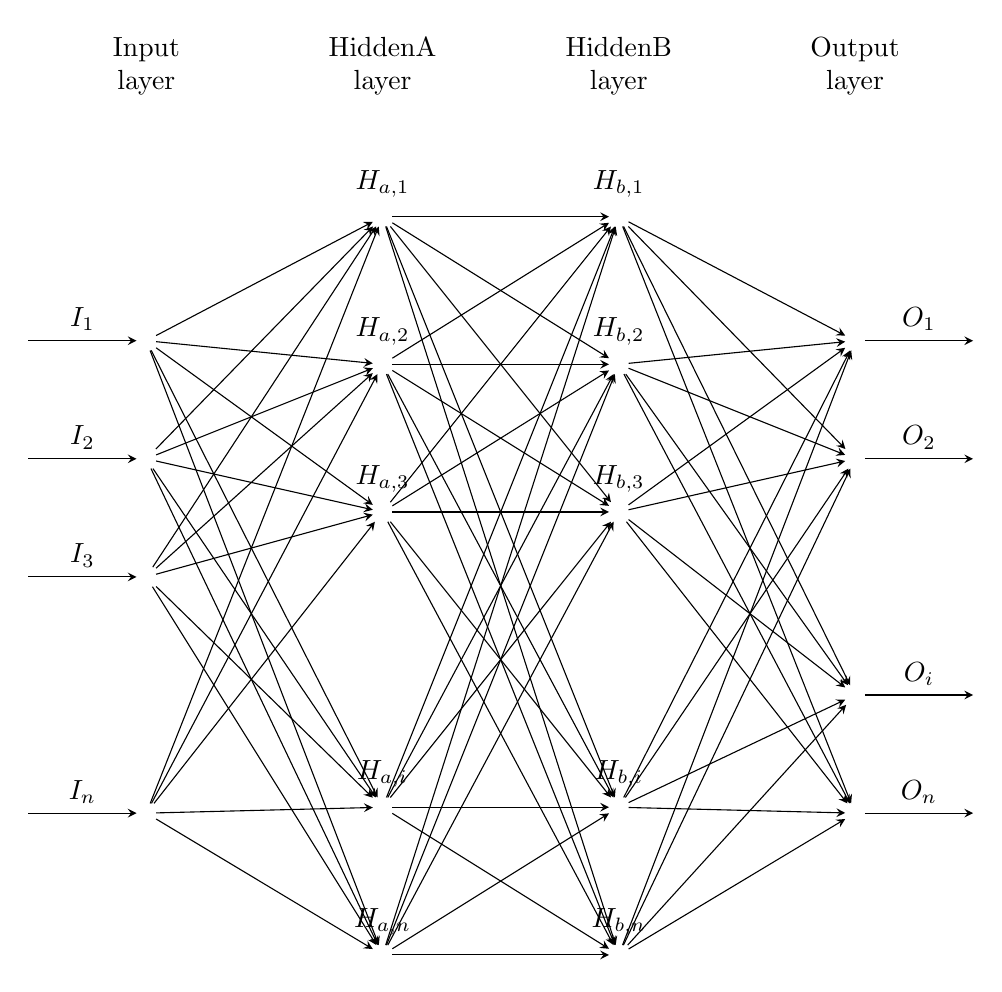
\begin{tikzpicture}[x=1.5cm, y=1.5cm, >=stealth]

    \foreach \m/\l [count=\y] in {1,2,3,missing,4}
      \node [every neuron/.try, neuron \m/.try] (input-\m) at (0,1-\y) {};
    
    \foreach \m [count=\y] in {1,2,3,missing,4,5}
      \node [every neuron/.try, neuron \m/.try ] (hiddenA-\m) at (2,2.3-\y*1.25) {};
    
    \foreach \m [count=\y] in {1,2,3,missing,4,5}
      \node [every neuron/.try, neuron \m/.try ] (hiddenB-\m) at (4,2.3-\y*1.25) {};
      
    \foreach \m [count=\y] in {1,2,missing,3,4}
      \node [every neuron/.try, neuron \m/.try ] (output-\m) at (6,1-\y) {};
    
    \foreach \l [count=\i] in {1,2,3,n}
      \draw [<-] (input-\i) -- ++(-1,0)
        node [above, midway] {$I_\l$};
    
    \foreach \l [count=\i] in {1,2,3,i,n}
      \node [above] at (hiddenA-\i.north) {$H_{a,\l}$};
    
    \foreach \l [count=\i] in {1,2,3,i,n}
      \node [above] at (hiddenB-\i.north) {$H_{b,\l}$};
    
    \foreach \l [count=\i] in {1,2,i,n}
      \draw [->] (output-\i) -- ++(1,0)
        node [above, midway] {$O_\l$};
    
    \foreach \i in {1,...,4}
      \foreach \j in {1,...,5}
        \draw [->] (input-\i) -- (hiddenA-\j);
    
    \foreach \i in {1,...,5}
        \foreach \j in {1,...,5}
            \draw [->] (hiddenA-\i) -- (hiddenB-\j);  

    \foreach \i in {1,...,5}
      \foreach \j in {1,...,4}
        \draw [->] (hiddenB-\i) -- (output-\j);
    
    \foreach \l [count=\x from 0] in {Input, HiddenA, HiddenB,Output}
      \node [align=center, above] at (\x*2,2) {\l \\ layer};
    
    \end{tikzpicture}
\end{center}
A network can be represented as a function $f$ parameterised by weight
matrix $\mathbf{W}$ and bias matrix $\mathbf{b}$ with the outputs of each
layer being passed into the next layer in a fully connected network.
\begin{equation}
    \mathbf{\hat{y}}= f(\mathbf{x}; \mathbf{W}, \mathbf{b})
\end{equation}
The network is optimised against a target output $Y$ using stochastic gradient descent.
\begin{equation}
    \begin{gathered}
        L(Y, \mathbf{\hat{y}}) = \Vert Y - \mathbf{\hat{y}} \Vert_{2} \\
        = \frac{1}{N} \cdot \sum_{i=1}^{N} (Y_i - (\mathbf{x}_i \cdot \mathbf{w}_i^\top + b))^2
    \end{gathered}
\end{equation}
\begin{equation}
    \begin{gathered}
        \frac{\partial E}{\partial \mathbf{w}} = -\frac{2}{N} \cdot \sum_{i=1}^{N} \mathbf{x}_i(Y_i-(\mathbf{x}_i \cdot \mathbf{w}_i^\top +b)) \\
    \frac{\partial E}{\partial b} = -\frac{2}{N} \cdot \sum_{i=1}^{N} (Y_i-(\mathbf{x}_i \cdot \mathbf{w}_i^\top +b))
    \end{gathered}
\end{equation}
\begin{gather}
    \begin{aligned}
        \nabla_{\mathbf{W}} E = \frac{\partial L(Y, \mathbf{\hat{y}}) }{\partial \mathbf{W}}  \,, \;\;\; &
        \nabla_{\mathbf{b}} E = \frac{\partial L(Y, \mathbf{\hat{y}})}{\partial \mathbf{b}} \,
    \end{aligned} 
\end{gather}
The error is calculated first for the network's output layers, the weights are then updated in the direction of 
negative gradient, steepest descent with respect to error $E$ with some constant stepsize $\eta$:
\begin{equation}
    \mathbf{W}_{k+1}=\mathbf{W}_{k} - \eta \nabla E_{\mathbf{W}_k}
\end{equation}
The gradients for the biases are updated likewise. This error is then back-propagated
using reverse mode differentiation on a computational graph \cite{Margossian2019} through the remaining nodes,
where the weights adjusted after the gradient updates are used as the target for the preceeding layer.
\begin{remark}
    In recent years additional properties of neural networks have been discovered
    relating to their nature as universal function approximators. Neural networks with
    a single hidden layer can approximate any function, and as the number
    of nodes tends to infinity it simplifies to a linear model \cite{Jaehoon2019}. Alternatively, infinitely
    wide, deep neural networks are equivalent to a gaussian process \cite{Jaehoon2017}.
    The have also demonstrated the ability to sort lists in practically $O(1)$ time \cite{Xiaoke2019}.
\end{remark}
\subsubsection{Deep Q-Networks}
Neural networks can be used to approximate the Q function directly using Q learning, however the structure
of the gradient update introduces complexity when trying to estimate expected value of rewards. We begin by 
parameterising our Q fuction with the weights of our network:
\begin{equation}
    \begin{gathered}
        Q(s,a)= f(\mathbf{s}; \mathbf{W}, \mathbf{b}) \;\;\;\; s \in \mathbf{S}\\
        \Rightarrow Q(s,a ; \mathbf{W}, \mathbf{b}) \rightarrow Q(s,a ; \mathbf{W}) \\
    \end{gathered}
\end{equation}
We can develop a loss function in the off policy setting using the Bellman Error $\delta_t$.
This holds because the update target $R_{t+1} + \gamma \max_a Q(S_{\textcolor{red}{t+1}},a)$ acts as a
"peek ahead" from the perspective of the current state. That is we take an action, observe the
outcome, and update the action-value of our old state with this new information.
\begin{equation}
    \begin{gathered}
        L(\delta_t, Q(s,a; \mathbf{W})) = \Vert \delta_t - Q(s,a; \mathbf{W}) \Vert_2 \\
        \frac{\partial L(\delta_t, Q(s,a;\mathbf{W} )) }{\partial \mathbf{W} } = \frac{\partial (\delta_t - Q(s,a; \mathbf{W}))^2}{\partial \mathbf{W}}\\
        = (\delta_t - Q(s,a; \mathbf{W})) \cdot \frac{\partial (\delta_t - Q(s,a; \mathbf{W}))}{\partial \mathbf{W}} \\
        = (\delta_t - Q(s,a; \mathbf{W})) \nabla_{\mathbf{W}} Q(s,a; \mathbf{W})
    \end{gathered}
\end{equation}
The target acts as a constant because the maximal estimated Q value at the next state is taken
to be the value of the state under the optimal policy (see 2.32). In their original paper, \cite{Mnih2015}
used a neural network to take in the state as input and then output a vector of action values, 
one for each action. If we used the intepretation of Q learning developed in (2.41), this structure could lead to unstable
gradient updates or could cause the action values to diverge. This can be described
in terms of the correlation between various elements of the model, consider
two dependent random variables $X$ and $Y$:
\begin{equation}
    \begin{gathered}
        Correlation(X,Y) = \frac{Covar(X,Y)}{\sqrt{Var(X)Var(Y)}} \\
        %Correlation(X,Y) \propto Covar(X,Y) \\
        %Correlation(X,Y) \propto \mathbb{E}[(X - \mathbb{E}[X])(Y - \mathbb{E}[Y])] \\
        %\propto \mathbb{E}[XY - X\mathbb{E}[Y] - Y\mathbb{E}[X] + \mathbb{E}[X]\mathbb{E}[Y]] \\
        %\propto \mathbb{E}[XY] - \mathbb{E}[X]\mathbb{E}[Y] - \mathbb{E}[Y]\mathbb{E}[X] + \mathbb{E}[X]\mathbb{E}[Y] \\
        %\propto \mathbb{E}[XY] - \mathbb{E}[X]\mathbb{E}[Y]\\
    \end{gathered}
\end{equation}
The corelation between two dependent random variables is proportional to the covariance of
the random variables normalised by their joint standard deviatiation $\sqrt{Var(X)}= \sigma$.
As correlation is a dimensionless constant on the interval $[-1,1]$, if $X$ and $Y$ are
correlated $Corr(X,Y) \approx 1$, then they increasingly co-vary across each dimension, then their
standard deviation must increase likewise, and as the co-variance goes to infinity, so does their
individual variance. And so under (2.41) we would be using a very similar distribution of
weights to calculate $\max_a Q(S_{t+1}, a)$ and $Q(S_{t}, a)$ which are both dependent 
according to the definition of our MDP. In addition to that, if we consider
successive frames of pixels on a screen as our states, it is trivial note that these
observations will also be highly correlated; in the case of the atari game "Pong", the
position on the paddle on the next frame is highly informed by position of the paddle in the next frame.

Instead, \cite{Mnih2015} propose two solutions to this problem. A biologically
inspired mechanism termed \emph{Experience Replay} and a separate \emph{Target Network}.
To remove the correlations between succesive observations $(S_t,A_t,R_{t+1},S_{t+1})$, they
instead store these tuples in a \emph{replay buffer}. In this case the replay buffer is a FIFO
array of constant size that overwrites older memories with new ones. The target network
is a seperate neural network whose weights $\theta^-$ are initialised with the weights of
the behaviour network and then frozen. Periodically, this target network is updated with the
current weights of the behaviour network $\theta$. 
Every timestep, a batch of memories are uniformly sampled, the target network is used to compute the Bellman Error
for each memory and the output of the behaviour network is updated according to the loss defined in (2.49),
averaged across the whole batch.
This algorithm proceeded to lead a breakthrough in contemporary deep reinforcment learning by outperforming
human benchmarks at a super human level for the first time (adapted from the original authors):
\begin{algorithm}[!htb]
    \SetAlgoLined
    \caption{Deep Q Network (DQN)}
    Init replay memory $D$ to capacity $N$ \;
    Init $Q$ with random weights $\theta$\;
    Init $\hat{Q}$ with $\theta^- = \theta$\;
    \ForAll{episodes}{
        Init state $s_1$\;
        Preprocess sequence $\phi_1 = \phi(s_1)$\;
        \ForAll{timesteps in episode}{
            $r \backsim U(0,1)$\;
            \eIf{r > $\varepsilon$}{
                $a_t \backsim {A}$ \tcp*[l]{ Randomly sample action from action space}
            }{
                $a_t = \underset{a}{argmax}\;\;Q(\phi(s_t),a ; \theta)$\;
            }
            Execute action $a_t$ observe $R_{t+1}, s_{t+1}, d$ \tcp*[l]{$d = 1$ if state is terminal else $0$} 
            Store $(\phi_1,a_t,r_{t+1},\phi_{t+1})$ in $D$\;
            Sampled random minibacth from $D$\;
            $\delta_t = r_t + (1-d) \gamma \max_{a'} \hat{Q}(\phi_{t+1},a'; \theta^-)$\;
            Perform gradient update $(\delta_t - Q(s,a; \theta)) \nabla_{\theta} Q(s,a; \theta)$\;
            Every $C$ steps reset $\hat{Q} = Q$\;
        }
    }
\end{algorithm}

\subsection{Improvements to Vanilla Deep Q-Networks}
Although the initial algorithm was very successful, it came with various stability 
issues arising from different sources. In particular, bootstraped values can be inherently
unstable \cite{sutton2018reinforcement} due to the nature of trying to estimate a guess from
a guess. Additionaly, sampling memories uniformly at random implicitly samples
are larger number of unsuccesful memories (i.e ones that did not attain a reward) than successful
memories as the action selections are initially random and uninformed at the start of training.
The na\"{i}ve $\varepsilon$ greedy policy is also prohibitive; it monotonic decrease across
the training run indicates that the exploration coefficient decreases for all states uniformly.
Another way of stating this is that no matter what state the agent is in, the likelihood
of choosing a random action to explore more of the state space decreases over time.
This may not be a desireable attribute, as we may want to explore more in some states over others,
and this preference for exploration may change over time as learn new information and update
our estimates (via bootstrapping). \\
In follow up work \cite{Hessel2017} combine subsequent improvements to the original DQN algorithm
addressing the issues listed above into a single agent termed the "Rainbow" agent. I will
go over each of the suggested improvements.
\subsubsection{Prioritised Experience Replay}
The motivation behind \emph{Prioritised Experience Replay} \cite{Schaul2015} is the notion that given
a batch of pre-recorded memories, the agent should ideally prioritise learning 
from certain experiences over others. Their work follows from neuroscientific studies
suggesting that the sequences of memories selected for experience replay in animals
are chosen proportionally to the rewards associated with that sequence and the magnitude of the
$\delta_t$ error. The magnitude of the $\delta_t$ error can be interpreted as the amount of "surprise"
associated with the that sequence, if our estimated Q value for a state action pair was far
from our target, the the result of our actions will always deviate from expectations because we did not
form a reliable way to ascertain the outcome of events. Updating our estimates for events in which
we were surprised is a necessary part of the learning cycle, and so prioritising memories according
to this surprise is warrented.\\
The authors assign a probability of being played to each memory as such:
\begin{equation}
    \begin{gathered}
        p_i = \vert \delta_i \vert + \epsilon \\
        P(i) = \biggl(\frac{p_i}{\sum_k p_k}\biggl)^\alpha
    \end{gathered}
\end{equation}
Where $\epsilon$ is some small positive constant to prevent the priority $p_i$ from being zero
and $P(i)$ is the probability of the transition being chosen for replay. The exponent $\alpha$
determines the amount of prioritisation used where $\alpha = 0$ is uniform (regular experience replay).
However the use of such a distribution introduces bias into the updates of the $Q$ value. The estimation
of an expected value with stochastic updates relies on those updates come from the same distribution as
our estimatiom, by construction the distribution as in (2.51), we are now drawing on observations
from a different distribution than the one underlying the MDP. This is corrected for with 
importance sampling weights introduced in \textbf{2.2.1.5}.
\begin{equation}
    \begin{gathered}
        w_i = \biggl(\frac{1}{N}\cdot \frac{1}{P(i)} \biggl)^\beta \\
        \nabla_\theta E = w_j \delta_j \nabla_\theta Q(S_{j-1}, A_{j-1}\:; \: \theta)
    \end{gathered}
\end{equation}
The bias is fully compensated for at $\beta = 1$ this ofcourse is coupled with a significant
increase in variance. In practice, the authors additionaly normalise the weights with $\frac{1}{\max_i w_i}$
so that the updates only scale downwards to reduce the overall magnitudes of the gradient updates
and $\beta$ is initialised to a low value $\backsim 0.4$ which is 
linearly annealed up to 1, this encourages additional stability during the training procedure.
The observations themselves are stored in a binary heap, specifically a \emph{Sum Segement Tree} rather
than a typical array or buffer:
\tikzset{
  treenode/.style = {align=center, inner sep=0pt, text centered,
    font=\sffamily},
  arn_n/.style = {treenode, circle, black, draw=black,
    text width=2em},% arbre rouge noir, noeud noir
  arn_r/.style = {treenode, circle, black, draw=black,
  text width=2em},% arbre rouge noir, noeud rouge
  arn_x/.style = {treenode, rectangle, draw=black,
    minimum width=0.5em, minimum height=0.5em}% arbre rouge noir, nil
}
\begin{figure}[!htb]
    \caption{Sum Segment Tree}
    \begin{center}
        \begin{tikzpicture}[->,>=stealth',level/.style={sibling distance = 5cm/#1,
            level distance = 1.5cm}] 
            
            \node [arn_n] {1}
            child{ node [arn_r] {0.33}
                        child{ node [arn_n] {0.15} 
                        }
                        child{ node [arn_n] {0.18}
                        }
                    }
                child{ node [arn_r] {0.67} 
                        child{ node [arn_n] {0.25} edge from parent node[above left]
                        {$0.67 - 0.42$} 
                        }
                        child{ node [arn_n] {0.42}
                        }  
                        edge from parent node[above right]
                        {$1 - 0.33$}                           
                }
                
            ; 
            \end{tikzpicture}
    \end{center}
\end{figure}
This offers the added benefit of $O(1)$ max priority read, the root of the tree, and 
$O(log N)$ time to update the priorities of each transition which resides on the leaves of
the tree. To traverse the tree for a batch size of $k$ memories, the interval $[0, p_{total}]$ is divided into $k$ equal intervals.
Each of these intervals is then uniformly sampled to produce a priority in that interval. The
transition whose value is the closest to each sampled priority is then chosen for replay by succesively
subtracting results until you arrive at a leaf as least as big as the query. Using this binary heap structure eliminates the
need for sorting, enabling the speed up in time complexity.
\subsubsection{Dueling Networks}
\cite{Ziyu2015} observed that the action value function can be decomposed
further into a value and advantage function:
\begin{equation}
    Q(s,a) = V(s) + A(s,a)
\end{equation}
Where the advantage is a measure of the advantage of taking an action in that state relative
to other possible actions. The expected value of a state is an estimate that takes into account
all possible action values of that state. Given than some values will be more valuable than others,
the expected value of a state can be taken to represent the weighted mean of all action values. Therefore
the maximal value of the optimal action of a state, will be greater than the mean, this difference is 
expressed as the advantage of that action. Ofcourse, in an optimal setting:
\begin{equation}
    \begin{gathered}
        A(s,a) = 0 \Longleftrightarrow V^*(s) = \max_a Q^*(s,a)\\
        \rightarrow A(s,a) = Q^*(s,a) - V^*(s) = 0
    \end{gathered}
\end{equation}
As the value of a state is the value of the most optimal action, the relative advantage of
the action to itself is $0$. Given only a $Q$ function we cannot recover the value
and advantage and value uniquely due to the nature of the inter-connectedness of the neural
network. Changes in the weights affect the entire space of approximation. Instead
the authors decompose the output layer of the DQN into two seperate heads, one that calculates
the advantage and another to calculate the value (as a scalar).

\definecolor{olivegreen}{rgb}{0,0.6,0}
\begin{figure}[!htb]
    \caption{Dueling Network Heads}
    \begin{center}
        \begin{tikzpicture}

            \path[rounded corners, fill=blue, fill opacity=0.2] (-0.4, 3.5) --  (-0.4, -3.5) -- (4, -3.5) -- (4, -0.2) -- (5, -0.2) -- (5, 3.5) -- (-0.4, 3.5) -- (-0.4, 0);
            \path[rounded corners, fill=red, fill opacity=0.2] (-0.4, -3.5) --  (-0.4, 3.5) -- (4, 3.5) -- (4, -0.2) -- (5, -0.2) -- (5, -3.5) -- (-0.4, -3.5) -- (-0.4, 0);
            \path[rounded corners, fill=white] (-0.4, 0) -- (-0.4, -3.5) -- (4, -3.5) -- (4, 3.5) -- (-0.4, 3.5) -- (-0.4, 0);
            \path[rounded corners, fill=olivegreen, fill opacity=0.2] (-0.4, 0) -- (-0.4, -3.5) -- (4, -3.5) -- (4, 3.5) -- (-0.4, 3.5) -- (-0.4, 0);
            \path [draw, dashed, very thick, rectangle, rounded corners] (-0.4, 0) -- (-0.4, -3.5) -- (5, -3.5) -- (5, 3.5) -- (-0.4, 3.5) -- (-0.4, 0);
            
            \node[circle, thick, fill=white, draw] (x1) {};
            \node[circle, thick, draw, fill=white, below=1em of x1] (x2) {};
            \node[circle, thick, fill=white, draw, below=1em of x2] (x3) {};
            \node[circle, thick, fill=white, draw, below=1em of x3] (x4) {};
            \node[circle, thick, fill=white, draw, below=1em of x4] (x5) {};
            \node[circle, thick, fill=white, draw, above=1em of x1] (x6) {};
            \node[circle, thick, fill=white, draw, above=1em of x6] (x7) {};
            \node[circle, thick, fill=white, draw, above=1em of x7] (x8) {};
            \node[circle, thick, fill=white, draw, above=1em of x8] (x9) {};
            \node[circle, thick, right=4em of x1, fill=white, draw] (xhh1) {};
            \node[circle, thick, draw, fill=white, below=1em of xhh1] (xhh2) {};
            \node[circle, thick, fill=white, draw, below=1em of xhh2] (xhh3) {};
            \node[circle, thick, fill=white, draw, below=1em of xhh3] (xhh4) {};
            \node[circle, thick, fill=white, draw, above=1em of xhh1] (xhh5) {};
            \node[circle, thick, fill=white, draw, above=1em of xhh5] (xhh6) {};
            \node[circle, thick, fill=white, draw, above=1em of xhh6] (xhh7) {};
            \node[circle, thick, right=8em of x1, fill=white, draw] (xh1) {};
            \node[circle, thick, draw, fill=white, below=1em of xh1] (xh2) {};
            \node[circle, thick, fill=white, draw, below=1em of xh2] (xh3) {};
            \node[circle, thick, fill=white, draw, below=1em of xh3] (xh4) {};
            \node[circle, thick, fill=white, draw, above=1em of xh1] (xh5) {};
            \node[circle, thick, fill=white, draw, above=1em of xh5] (xh6) {};
            \node[circle, thick, fill=white, draw, above=1em of xh6] (xh7) {};
            \node[circle, very thick, fill=blue!30, draw, right=12em of x1, yshift=5em] (hm1) {};
            \node[circle, very thick, draw, fill=blue!30, below=0.5em of hm1] (hm2) {};
            \node[circle, very thick, draw, fill=blue!30, below=0.5em of hm2] (hm3) {};
            \node[circle, very thick, draw, fill=blue!30, above=0.5em of hm1] (hm4) {};
            \node[circle, very thick, draw, fill=blue!30, above=0.5em of hm4] (hm5) {};
            \node[circle, very thick, fill=red!30, draw, right=12em of x1, yshift=-5em] (hs1) {};
            \node[right=1.5em of hm1, blue] (mu1) {$A_{\theta_1}(s, \alpha_3)$};
            \node[right=1.5em of hm2, blue] (mu2) {$A_{\theta_1}(s, \alpha_4)$};
            \node[right=1.5em of hm3, blue] (mu3) {$A_{\theta_1}(s, \alpha_5)$};
            \node[right=1.5em of hm4, blue] (mu4) {$A_{\theta_1}(s, \alpha_2)$};
            \node[right=1.5em of hm5, blue] (mu5) {$A_{\theta_1}(s, \alpha_1)$};
            \node[right=1.5em of hs1, red] (s1) {$V_{\theta_2}(s)$};
                
            \foreach \x in {1,...,9}
                \foreach \y in {1,...,7}
                    \draw[-stealth, thick] (x\x) -- (xhh\y);
            
            \foreach \x in {1,...,7}
                \foreach \y in {1,...,7}
                    \draw[-stealth, thick] (xhh\x) -- (xh\y);
            
            \foreach \x in {1,...,7}
                \foreach \y in {1,...,5}
                    \draw[-stealth, thick, blue] (xh\x) -- (hm\y);
            
            \foreach \x in {1,...,7}
                \draw[-stealth, thick, red] (xh\x) -- (hs1);
            
            \draw[-stealth, decoration={snake, pre length=0.01mm, segment length=2mm, amplitude=0.3mm, post length=1.5mm}, decorate, thick, red] (hs1) -- (s1);
            
            \foreach \x in {1,...,5}
                \draw[-stealth, decoration={snake, pre length=0.01mm, segment length=2mm, amplitude=0.3mm, post length=1.5mm}, decorate, thick, blue] (hm\x) -- (mu\x);
                        
            \node[left=0.75em of x1] (l1) {$s$};
        \end{tikzpicture}
    \end{center}
    \scriptsize{\dag Source: \url{https://github.com/PetarV-/TikZ/blob/master/A3C\%20neural\%20network/a3c_neural_network.tex} }
\end{figure}
The action value is then calculated:
\begin{equation}
    Q(s,a \: ; \: \theta) = V(s\:;\:\theta_2 ) + (A(s,a\:;\:\theta_1) - \mathbb{E}[A(s,a\:;\:\theta_1)])
\end{equation}
One can fix this lack of identifiability by forcing the function approximator to maximise the
value of the state by having a 0 advantage at the chosen action, hence we subtract the mean.
The $Q$ values for bothe the behaviour and target network are calculated this way.
\subsubsection{Double Q Learning }
Consider the MDP given by fig (2.10),
\begin{figure}[!htb]
    \caption{Maximization Bias Example}
    \begin{center}
        \begin{tikzpicture}[auto,node distance=8mm,>=latex,font=\small]

            \tikzstyle{round}=[thick,draw=black,circle]
        
            \node[round] (s0) {$A$};
            \node[round, right=0mm and 20mm of s0] (s1) {$T_1$};
            \node[round, left=0mm and 20mm of s0] (s2) {$B$};
            \node[round, left=0mm and 20mm of s2] (s3) {$T_2$};
            \draw[->]  (s0) -- (s1) node [midway, above]{$0$};
            \draw[->] (s0) -- (s2) node [midway, above]{$0$};
            \draw[->] (s2.north) to [out=110,in=70] node[above]{$\mathcal{N}(-0.1,1)$} (s3.north);
            \draw[->] (s2) -- (s3) node [midway, above]{$\vdots$} node [midway, below]{$\vdots$};
            \draw[->] (s2.south) to [out=-110,in=-70] node[below]{} (s3.south);
        \end{tikzpicture}
    \end{center}
    \scriptsize{\dag Source: \cite{sutton2018reinforcement}}
\end{figure}
the agent begins in state A and can either move left or right for a reward in 0.
Moving right will terminate the process with reward 0. Moving left (with reward 0)
puts the agent in a state where it can choose amongst a multitude of actions whose
rewards are normaly distributed with a mean of -0.1 and variance of 1.
During policy iteration we select actions according to $\underset{a}{argmax} \: Q(s,a)$,
this incurs a significant \emph{positive} bias due to the nature of the maximization, in
fig (2.10) the agent will always choose the left action as it seeks to maximise the expected
return and certain returns from going to $B$ will be greater than 0; instead the agent should
choose to go right, because the expected value of that action is greater
than the expected value of going to $B \backsim -0.1$.
The error occurs because the same samples are used to determine both the value of each action and to select
the maximising action. \cite{Hasselt2015} address this within the context of deep Q learning
by proposing the following variant of the temporal difference $\delta_t$ error:
\begin{equation}
    y_i = R_{t+1} + \gamma Q(S_{t+1}, \underset{a}{argmax} \: Q(S_{t+1}, A_{t+1}\:;\:\theta)\:;\: \theta^-)
\end{equation}
The Q value of the next state is calculated first by finding the most optimal action for
that next state according to our behaviour policy parameters $\theta$ and then selecting
the Q value of the action according to its value under the target network's parameters $\theta^-$.
By doing so we decouple the estimation of an actions value from its selection. The authors
show that this is effective in combination with the previously discussed improvements.
\subsubsection{Distributional Reinforcement Learning}
Recalling equation (2.41), the expected future discounted reward is a weighted mean,
whose final output is a scalar value. This mean ignores the variance and possible multi-modality
of the underlying distribution. Assuming that the process of generalized policy iteration
reaches a fixed point $\pi^* = \pi_\theta$ where the policy under the neural network's parameters
aproximates the optimal policy arbitarily well, this approximation is only in their means, and equality
of means does not gurantee that the "shape" of the underlying distributions are the same.
Motivated by these shortcomings, \cite{Bellemare2017} proposed an alternative distributional perspective
on reinforcement learning. The authors reinterpret equation (2.41) under a distributional variant;
first they contextualize the Q learning update under the \emph{Bellman operator} $\mathcal{T}^\pi$ and in the control setting
as the application of the \emph{"optimality operator"} $\mathcal{T}$:
\begin{equation}
    \begin{gathered}
        x \in \mathbf{S}, \;\; x' \coloneqq x_{t+1}\\
        \mathcal{T}^\pi Q(x,a) = \mathbb{E}[R(x,a)] + \gamma \underset{P,\pi}{\mathbb{E}} [Q(x',a')] \\
        \rightarrow \mathcal{T} Q(x,a) = \mathbb{E}[R(x,a)] + \gamma \underset{P,\pi}{\mathbb{E}} [\max_{a' \in A}Q(x',a')]
    \end{gathered}
\end{equation}
This reflects the same objective as (2.41), where successive applications of the Bellman operator
produce new policies paramterised by the updated estimates to the Q value function. Additionally we recognise
that the reward $R(x,a)$ the agent receives depends on the action taken in that particular state. Under the
distributional setting the state is denoted $x' \backsim P( \cdot \mid x, a)$ as the state is assumed
to be sampled from the underlying steady state distribution of the MDP\footnote{See equation (2.41)}.
Considering the markov property\footnote{See \textbf{2.2.1}}, the discounted future returns $\gamma G_{t+1}$ of a particular state
can be considered a random variable $Z$ distrbuted according to the probability of attaining
certain returns dependent on the action taken in each state, formally $R \in \mathbf{Z}$, where
$\mathbf{Z}$ represents a mapping from state-action pairs to \emph{distributions} of returns.
Furthermore the authors describe "transition operator" as an operator that transforms the current
distribution of discounted returns into the distribution of discounted returns for the next state:
\begin{equation}
    \begin{gathered}
        \mathcal{P}^\pi : Z \mapsto Z'\\
        \mathcal{P}^\pi Z(x,a) \distributed Z(x',a') \\
        x' \backsim P(\cdot \mid x,a), \;\; a' \backsim \pi(\cdot \mid x')
    \end{gathered}
\end{equation}
In this case, the transition operator will map the distribution
of returns under the current state and action, to the distribution returns under the next state action  pair which
is distributed according to the same law (denoted by $\distributed$) as the previous distribution. They then
reformulate the Bellman operator:
\begin{equation}
    \begin{gathered}
        \mathcal{T}^\pi Z(x,a) \distributed R(x,a) + \gamma \mathcal{P}^\pi Z(x,a)
    \end{gathered}
\end{equation}
Three sources of randomness arise under this interpretation:
\begin{itemize}
    \item Randomness in reward $R(x,a)$.
    \item Randomness in the transition $\mathcal{P}^\pi$.
    \item Randomness in the next state-value distribution $Z(x',a')$.
\end{itemize}
These sources are important to observe when considering if the distributional variant of the Bellman equation
converges to a fixed point $Z^\pi$. In order to measure the relative distance between an arbitary distribution,
the authors utilise the \emph{Wasserstein} distance defined on cumulative density functions (c.d.f) of arbitary probability
density functions (p.d.f). If a random variable is distributed according to $F(x)$ then it's c.d.f, also known
as a quantile function, is $F^{-1}(x)$. The \emph{Wasserstein} distance is an $L_p$ metric for some $p \in \mathbb{N}$ that measures the distance
between two random variables $U, V$ on the space of possible samples (values the variable can take on) $\omega \in \Omega$
is the smallest possible difference between the probability density of each sample whose support is the metric space $[0,1]$:
\begin{equation}
    \begin{gathered}
        W_p(F,G) = \biggl ( \int_{0}^{1} \vert F^{-1}_U(\omega) - F^{-1}_{V}(\omega) \vert^p \,\mathrm{d}x \biggl )^{\frac{1}{p}} \\
        = \inf_{U,V} \Vert U - V \Vert_p
    \end{gathered}
\end{equation}
To measure the distance between value distributions $Z_1, Z_2$, they define the maximal form of the Wasserstein metric
as the highest element-wise absolute difference between the two:
\begin{equation}
    \bar{d}_p(Z_1, Z_2) \coloneqq \sup_{x,a} W_p(Z_1(x,a), Z_2(x,a)) 
\end{equation}
The authors show that similarly to equation (2.20) the $\bar{d}_p$ metric is a contraction in $\gamma$
by \emph{Banach's fixed point theorem}:
\begin{equation}
    \begin{gathered}
        \bar{d}_p( \mathcal{T}^\pi Z_1, \mathcal{T}^\pi Z_2) \leqslant \bar{d}_p(R + \gamma \mathcal{P}^\pi Z_1, R + \gamma \mathcal{P}^\pi Z_2) \\
        \leqslant \bar{d}_p(\gamma \mathcal{P}^\pi Z_1, \gamma \mathcal{P}^\pi Z_2) \\
        \leqslant \vert \gamma \vert \bar{d}_p(\mathcal{P}^\pi Z_1, \mathcal{P}^\pi Z_2) \\
        \leqslant \gamma \bar{d}_p(Z_1, Z_2) 
    \end{gathered}
\end{equation}
In theory, these results can be applied directly by substituting (2.56) for the Q learning update, however
the issue arises when incorporating function approximation in an effort to parameterise the distribution
of returns for each state-action pair. Starting from random, the network's parameters 
are continually updated to more closely reflect the actual distribution of returns for each state action pair.
As a result, the support\footnote{Range of values that the expected discounted return of a state action pair can take on with a non-zero probability}
of the predicted distribution, the output of the neural network, will drift over time. Generalised policy iteration
continuously produces new policies, in this case, the result is that each policy is defined on a different support.
This poses an issue, as the distance between two random variables on disjoint supports is infinite \cite{Bellemare2017}.
In practice the authors overcome this by utilising a $\mathbf{\Phi}_2$ projection of the output distribution of the network 
onto a discrete support with $N$ atoms and then minimzing the \emph{Kullback Liebler} divergence between the target and the prediction.\\

However as \cite{Dabney2017} note in their follow up work, the conjugation of the $\mathbf{\Phi}_2$ operator with the Bellman operator $\mathcal{T}^\pi$
does not necessarily converge to the \emph{same fixed point} as the repeated application of the $\mathcal{T}^\pi$. Additionally, in practice
the $\mathbf{\Phi}_2$ projection requires conducting a nearest neighbour search between the atoms of the predicted distribution
and the target distribution, and assigning credit proportionally to the 2 nearest neighbours, this can be unwieldy to implement.
\cite{Dabney2017} instead propose \emph{quantile regression} as a way around these limitations.\\

Where \cite{Bellemare2017} choose to fix the support and vary the probabilities,\cite{Dabney2017} invert
this formulation to instead fix the probabilities and vary the support. The complete metric space of
probability $[0,1]$ is discretized into $\tau$ uniform intervals and the appropriate density of returns 
is allocated to each interval. First they show that the projection $\Pi_{W_1}$ of any arbitary value distribution
$Z$ onto a distribution of $\tau$ number of quantiles $Z_Q$, preserves the convergence to a fixed point under the conjugation
of $\bar{d}_p \circ \Pi_{W_1}$:
\begin{equation}
    \bar{d}_p(\Pi_{W_1} \mathcal{T}^\pi Z_1,\Pi_{W_1} \mathcal{T}^\pi Z_2) \leqslant \gamma \bar{d}_p(Z_1, Z_2)
\end{equation}
The Q network aims to predict the quantiles $\theta_i$ for each action  resulting in a vector $Z_\theta \in Z_Q$
for each action such that $Z_{\theta_i} = P(y_i < \theta_i)$\footnote{For instance if $\tau = 6$ then $Z_{\theta_5} = y_i$ s.t $P(y_i < Q(\frac{5}{6})) \mid  F^{-1}(Q(\frac{5}{6})) = \frac{5}{6}$}. 
In order to project an arbitary distribution onto a distribution of $N$ quantiles
it follows that the most suitable distribution is that which minizes the \emph{Wasserstein} metric $\Pi_{W_1}Z= \arg \min W_p(Z, Z_Q)$. 
The authors show that the value on the interval of each quantile that minimizes this distance is the
median of the interval:
\begin{equation}
    \begin{gathered}
        \arg \min \int^{\tau'}_\tau \vert F^{-1}(\omega) - \theta \vert \, d\omega \\
        \text{Is given by} \\
        \theta : F(\theta) = \frac{\tau + \tau'}{2}
    \end{gathered}
\end{equation}
They utilise \emph{quantile regression loss} developed within economics, to fit the predicted
quantile distribution of action-values to a target quantile distribution. Formally, a dirac delta
function positioned on the quantile is scaled proportionally when the distance $\xi = \hat{Z} - \theta$ 
is overestimated $\xi \geq 0$ or underestimated $\xi < 0$. Quantile regression is used
to fit the predicted quantile to the target by minimizing the following objective:
\begin{equation}
    \begin{gathered}
        \rho_\tau(u) = \begin{cases}
            \tau \cdot u & u \geq 0 \\ %Update this!
            (1 - \tau) \cdot u & u < 0
        \end{cases} \\
        \mathcal{L}^\tau_{QR} \coloneqq  \sum_{i=1}^N \E_{\hat{Z} \backsim Z}[\rho_\tau(\hat{Z} -\theta_i)]
    \end{gathered}
\end{equation}
This is in turn applied to the Bellman update: 
\begin{equation}
    \begin{gathered}
        \mathcal{T}Q(x,a) = \mathbb{E}[R(x,a)] + \gamma \mathbb{E}_{z' \backsim P}[\max_{a'}Q(x',a')] \\
        \rightarrow \mathcal{T}Z(x,a) = R(x,a) + \gamma Z(x',a') \\
        x' \backsim P(\cdot \mid x,a), a' = \arg \max_{a'} \mathbb{E}_{z \backsim Z(x',a')}[z] \\
    \end{gathered}
\end{equation}
From which the authors derive the TD control update:
\begin{equation}
    \theta_i(x) \leftarrow \theta_i(x) + \alpha(\hat{\tau}_i - \delta_{r + \gamma < \theta_i(x)})
\end{equation}
\cite{Dabney2017} results show that learners that incorporate the distribution of returns (\textbf{risk-sensitive learners})
perform much better and converge to optimal policies much faster, this increase in performance is no doubt
due to the greater representational power of distributions.